\subsection{Medidas de Avaliação em Segmentação Textual}


% 


As medidas de avaliação tradicionais como precisão e revocação são permitem medir o desempenho de modelos de Recuperação de Informação e Aprendizado de Máquina por meio da comparação dos valores produzidos pelo modelo com os valores observados em uma referência. 
%	Avaliações baseadas em hits 
Usa-se uma tabela, chamada matriz de confusão, para visualizar o desempenho de um algoritmo. Na Tabela~\ref{tab:matrizconfusao} é apresentada uma matriz de confusão para duas classes (Positivo e Negativo). 

\begin{table}[!h]
\centering

\begin{tabular}{|c|c|c|}
  \hline
				& Predição Positiva        & Predição Negativa        \\ \hline
  Positivo real & VP (Verdadeiro Positivo) & FN (Falso Negativo)      \\ \hline
  Negativo real & FP (Falso Positivo)      & VN (Verdadeiro Negativo) \\ \hline

\end{tabular}

\caption{Matriz de confusão.}
\label{tab:matrizconfusao}

\end{table}


%
% Falso Positivo 
% Falso Negativo 
% Verdadeiro Positivo 
% O Verdadeiro Negativo, que não existe 
%%% 
No contexto de segmentação textual, um falso positivo é um limite identificado pelo algoritmo que não corresponde a nenhum limite na segmentação de referência, ou seja, o algoritmo indicou que em determinado ponto há uma quebra de segmento, mas na segmentação de referência, no mesmo ponto, não há. De maneira semelhante, um falso negativo é quando o algoritmo não identifica um limite existente na segmentação de referência, ou seja, em determinado ponto há, na segmentação de referência, um limite entre segmentos, contudo, o algoritmo não o identificou.  Um verdadeiro positivo é um ponto no texto indicado pelo algoritmo e pela segmentação de referência como uma quebra de segmentos, ou seja, o algoritmo e a referência concordam que em determinado ponto há uma transição de assunto.  Na avaliação de segmentadores, não há o conceito de verdadeiro negativo. Este seria um ponto no texto indicado pelo algoritmo e pela segmentação de referência onde não há uma quebra de segmentos. Uma vez que os algoritmos apenas indicam onde há um limite, essa medida não é necessária. % Não há ou não e necessário?


% 
% Precisão 
%%%
Nesse sentido, a precisão indica a proporção de limites corretamente identificados pelo algoritmo, ou seja, correspondem a um limite real na segmentação de referência. 
Porém, não diz nada sobre quantos limites reais existem. 
É calculada dividindo-se o número de limites identificados automaticamente pelo número de candidatos a limite (Equação~\ref{equ:precisao}).
 
 \begin{equation}
	 Precis\tilde{a}o = \frac{VP}{VP+FP}
	 \label{equ:precisao}
 \end{equation}

%
% Revocação 
%%%
 A revocação, é a proporção de limites verdadeiros que foram identificados pelo algoritmo. Porém não diz nada sobre quantos limites foram identificados incorretamente. É calculada dividindo-se o número de limites identificados automaticamente pelo número limites verdadeiros (Equação~\ref{equ:revocacao}).
 
 \begin{equation}
	 Revoca\c{c}\tilde{a}o = \frac{VP}{VP+FN}
	 \label{equ:revocacao}
 \end{equation}

 Existe uma relação inversa entre precisão e revocação. Conforme o algoritmo aponta mais segmentos no texto, este tende a melhorar a revocação e ao mesmo tempo, reduzir a precisão. Esse problema de avaliação pode ser contornado utilizado a medida $F^1$ que é a média harmônica entre precisão e revocação onde ambas tem o mesmo peso (Equação~\ref{equ:f1}). 

 \begin{equation}
	 F^1 = \frac{2 \times Precis\tilde{a}o \times Revoca\c{c}\tilde{a}o}
		        {Precis\tilde{a}o + Revoca\c{c}\tilde{a}o}
	 \label{equ:f1}
 \end{equation}



%-> Precisão é a fração de instâncias recuperadas que são relevantes, 
%-> Revocação é a fração de instâncias relevantes que são recuperadas.
%-> https://pt.wikipedia.org/wiki/Precis%C3%A3o_e_revoca%C3%A7%C3%A3o





























As medidas de avaliação tradicionais como precisão e revocação permitem medir o desempenho de modelos de Recuperação de Informação e Aprendizado de Máquina por meio da comparação dos valores produzidos pelo modelo com os valores observados em uma referência. 
%	Avaliações baseadas em hits 
Usa-se uma tabela, chamada matriz de confusão, para visualizar o desempenho de um algoritmo. Na Tabela~\ref{tab:matrizconfusao} é apresentada uma matriz de confusão para duas classes (Positivo e Negativo). 


\begin{table}[!h]
\centering

\begin{tabular}{|c|c|c|}
  \hline
				& Predição Positiva        & Predição Negativa        \\ \hline
  Positivo real & VP (Verdadeiro Positivo) & FN (Falso Negativo)      \\ \hline
  Negativo real & FP (Falso Positivo)      & VN (Verdadeiro Negativo) \\ \hline

\end{tabular}

\caption{Matriz de confusão.}
\label{tab:matrizconfusao}

\end{table}


% -> Falso Positivo % Falso Negativo % Verdadeiro Positivo % O Verdadeiro Negativo, que não existe 

No contexto de segmentação textual, um falso positivo é um limite identificado pelo algoritmo que não corresponde a nenhum limite na segmentação de referência, ou seja, o algoritmo indicou que em determinado ponto há uma quebra de segmento, mas na segmentação de referência, não há quebra no mesmo ponto. De maneira semelhante, um falso negativo é quando o algoritmo não identifica um limite existente na segmentação de referência, ou seja, em determinado ponto há, na segmentação de referência, um limite entre segmentos, contudo, o algoritmo não o identificou.  Um verdadeiro positivo é um ponto no texto indicado pelo algoritmo e pela segmentação de referência como uma quebra de segmentos, ou seja, o algoritmo e a referência concordam que em determinado ponto há uma transição de assunto.  Na avaliação de segmentadores, não há o conceito de verdadeiro negativo. Este seria um ponto no texto indicado pelo algoritmo e pela segmentação de referência onde não há uma quebra de segmentos. Uma vez que os algoritmos apenas indicam onde há um limite, essa medida não é necessária. % Não há ou não e necessário?


% -> Precisão 
Nesse sentido, a precisão indica a proporção de limites corretamente identificados pelo algoritmo, ou seja, correspondem a um limite real na segmentação de referência. 
Porém, não diz nada sobre quantos limites reais existem. 
É calculada dividindo-se o número de limites identificados automaticamente pelo número de candidatos a limite (Equação~\ref{equ:precisao}).
 
 \begin{equation}
	 Precis\tilde{a}o = \frac{VP}{VP+FP}
	 \label{equ:precisao}
 \end{equation}


% -> Revocação 

 A revocação, é a proporção de limites verdadeiros que foram identificados pelo algoritmo. Porém não diz nada sobre quantos limites foram identificados incorretamente. É calculada dividindo-se o número de limites identificados automaticamente pelo número limites verdadeiros (Equação~\ref{equ:revocacao}).
 
 \begin{equation}
	 Revoca\c{c}\tilde{a}o = \frac{VP}{VP+FN}
	 \label{equ:revocacao}
 \end{equation}

 Existe uma relação inversa entre precisão e revocação. Conforme o algoritmo aponta mais segmentos no texto, este tende a melhorar a revocação e ao mesmo tempo, reduzir a precisão. Esse problema de avaliação pode ser contornado utilizado a medida $F^1$ que é a média harmônica entre precisão e revocação onde ambas tem o mesmo peso (Equação~\ref{equ:f1}). 

 \begin{equation}
	 F^1 = \frac{2 \times Precis\tilde{a}o \times Revoca\c{c}\tilde{a}o}
		        {Precis\tilde{a}o + Revoca\c{c}\tilde{a}o}
	 \label{equ:f1}
 \end{equation}



%-> Precisão é a fração de instâncias recuperadas que são relevantes, 
%-> Revocação é a fração de instâncias relevantes que são recuperadas.
%-> https://pt.wikipedia.org/wiki/Precis%C3%A3o_e_revoca%C3%A7%C3%A3o

% =============================================================


%  Medidas de avaliação tradicionais 
As medidas de avaliação tradicionais, precisão e revocação, podem não ser confiáveis, por não considerarem a distância entre os limites, mas penalizam o algoritmo sempre que um limite que não coincide perfeitamente com a referência. Essas medidas podem ser mais adequadas quando necessita-se de segmentações com maior exatidão. Em outras palavras, computam apenas os erros do algoritmo quando se detecta falsos positivos ou falsos negativos, o que nesse contexto de segmentação textual pode não ser suficiente, dado a subjetividade da tarefa. Além dessas medidas, que consideram apenas se um segmento foi perfeitamente definido conforme uma referência, pode-se também considerar a distância entre o segmento extraído automaticamente e o segmento de referência~\cite{Kern2009}. Chama-se \textit{near misses} o caso em que um limite identificado automaticamente não coincide exatamente com a referência, mas é necessário considerar a proximidade entre eles.

%  Medidas que consideram a distancia entre os segmentos 
Na Figura~\ref{fig:exemplosegmentacaozoom} é apresentado um exemplo com duas segmentações extraídas automaticamente e uma referência. Em ambos os casos não há nenhum verdadeiro positivo, o que implica em zero para os valores de precisão, acurácia, e revocação, embora o resultado do algoritmo A possa ser considerado superior ao primeiro se levado em conta a proximidade dos limites.
% Para não confundir hipótese com algoritmo, escrever: "A hipótese A, produzida pelo algoritmo A e a hipótese B, produzida pelo algoritmo B".
% Ou trocar hipótese por resultado do algoritmo A, B

  \begin{figure}[!h]

	\centering
	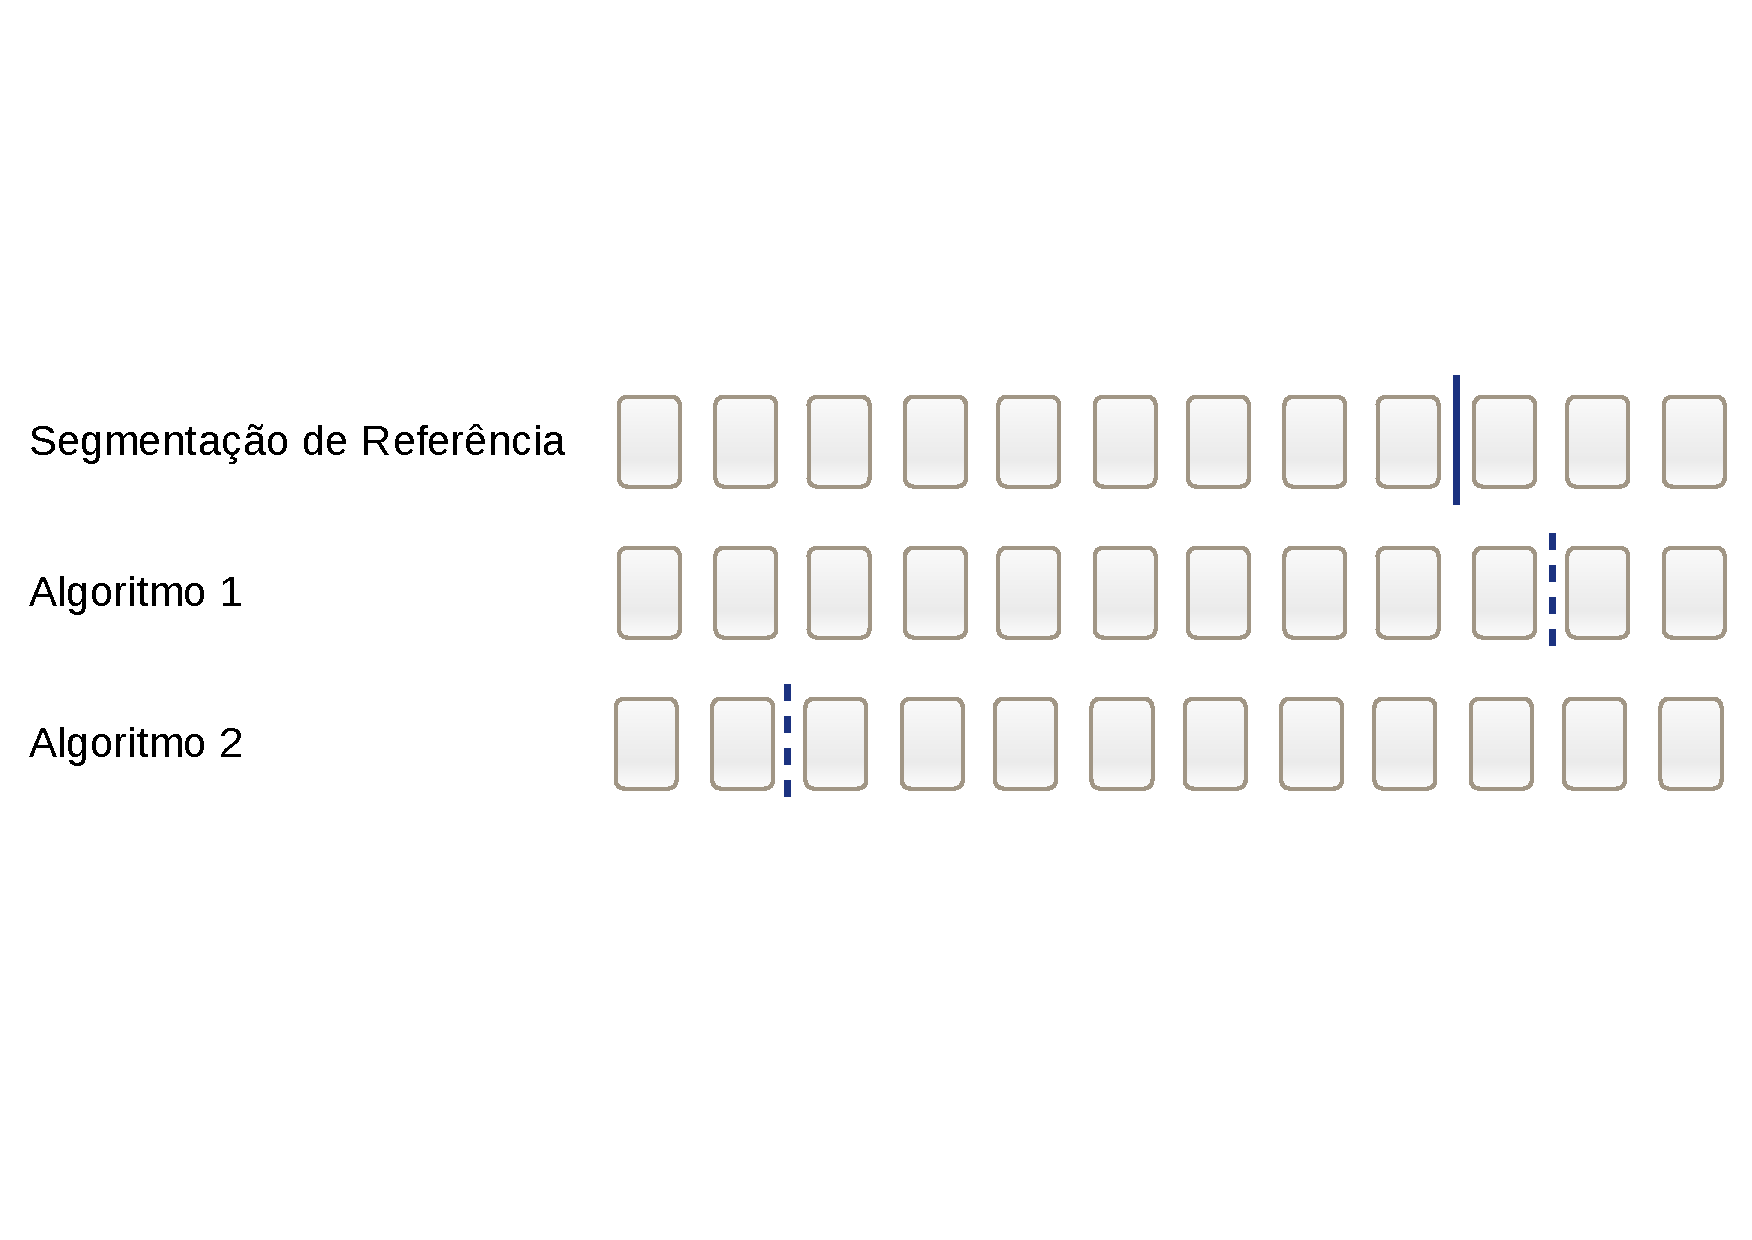
\includegraphics[trim={ 0 180 0 180 },clip,page=1,width=0.7\textwidth]{conteudo/capitulos/figs/near-missing.pdf}
	\caption{Exemplos de \textit{near missing} e falso positivo puro. Os blocos indicam uma unidade de informação e as linha verticais representam uma transição de assunto. }
	\label{fig:exemplosegmentacaozoom}

  \end{figure}
  


% === PK ===

Considerando o conceito de \textit{near misses}, algumas medidas de avaliação foram propostas. Proposta por~\cite{Beeferman1999}, P$_k$ atribui valores parciais a \textit{near misses}, ou seja, limites sempre receberão um peso proporcional à sua proximidade, desde que dentro de um janela de tamanho~$k$.  Para isso, esse método move uma janela de tamanho $k$ ao longo do texto. A cada passo verifica, na referência e no algoritmo, se as extremidades (a primeira e última sentença) da janela estão ou não dentro do mesmo segmento, então, penaliza o algoritmo caso este não concorde com a referência. Ou seja, dado dois termos de distância $k$, $P_k$ verifica se o algoritmo coloca os termos no mesmo segmento ou em segmentos distintos e o penaliza caso não concorde com a referência. Dadas uma segmentação de referência $ref$ e uma segmentação automática $hyp$, ambas com $N$ sentenças, P$_k$ é computada como:


\begin{equation}
P_k(ref,hyp) = \frac{1}{N - k}
\sum_{i=1}^{N-k } 
(
\delta_{ref}(i, i+k) ~
\bar{\oplus} ~
\delta_{hyp}(i, i+k) 
)
\end{equation}


onde $\delta_S(i,j)$ é a função indicadora que retorna 1 se as sentenças i e j estão no mesmo segmento e 0 caso contrário, $\bar{\oplus}$ é o operador \texttt{XNOR} (ambos ou nenhum) que retorna 1 se ambos os argumentos forem diferentes. 
%
%
O valor de $k$ é calculado como a metade da média dos comprimentos dos segmentos reais. Como resultado, é retornada a dissimilaridade entre a segmentação calculada pela contagem de discrepâncias divida pela quantidade de segmentos analisados. Essa medida pode ser interpretada como a probabilidade de duas sentenças extraídas aleatoriamente pertencerem ao mesmo segmento.  




% === WindowDiff ===

\textit{WindowDiff}~\cite{Pevzner2002} é uma medida alternativa à P$_k$. De maneira semelhante, move uma janela pelo texto e penaliza o algoritmo sempre que o número de limites proposto pelo algoritmo não coincidir com o número de limites esperados para aquela janela. Ou seja, o algoritmo é penalizado quando não concordar com a segmentação de referência quanto ao número de segmentos na janela. Mais formalmente, para cada intervalo $k$, compara o número de segmentos obtidos pela referência $r_i$ com o obtido pelo algoritmo $a_i$ e penaliza o algoritmo se $r_i \neq a_i$. Na Equação~\ref{equ:windiff} é mostrada a definição de WindowDiff onde $b(i, i+k)$ representa o número de limites entre as sentenças $i$ e $i+k$ e $N$, o total de sentenças no texto.
% e $k = \frac{N}{2 \times n\'{u}mero\ de\ segmentos}$. 

\begin{equation}
	WindowDiff(ref,hyp) = \frac{1}{N-k}\sum_{i=1}^{N-k}(|b(ref_i - ref_{i+k}) - b(hyp_i - hyp_{i+k})| > 0)
	\label{equ:windiff}
\end{equation}


Assim, consegue manter a sensibilidade a \textit{near misses} e além disso, considerar o tamanho das janelas.  A fim de melhor equilibrar o peso dos falsos positivos em relação a \textit{near misses}, dobra-se a penalidade para falsos positivos, evitando-se a supervalorização dessa medida.  % OBS: Os problemas de Pk ficaram subentendidos aqui :/ 

As medidas \textit{WindowDiff} e P$_k$, consideram a quantidade e proximidade entre os limites, sendo mais tolerantes a pequenas imprecisões. Essa é uma característica desejável, visto que as segmentações de referência possuem diferenças consideráveis. \textit{WindowDiff} equilibra melhor os falsos positivos em relação a \textit{near misses}, ao passo que P$_k$ os penaliza com peso maior. Isso significa que segmentadores melhores avaliados em P$_k$ ajudam a selecionar as configurações que erram menos ao separar trechos de texto com o mesmo assunto, enquanto \textit{WindowDiff} é mais tolerante nesse aspecto.  De maneira geral, observa-se  melhores resultados de \textit{WindowDiff} quando os algoritmos aproximam a quantidade de segmentos automáticos da quantidade de segmentos da referência. Por outro lado, P$_k$ avalia melhor as configurações que retornam menos segmentos. Contudo, não é possível definir um valor adequado, uma vez que os segmentadores humanos frequentemente apontam segmentações diferentes.


